\section{Data}\label{sec:data}

\subsection{Kalshi}

Kalshi is a regulated US exchange on which event contracts trade in a central limit order book, each contract paying \$1 if the event occurs. Table~\ref{tab:kalshi_series} lists the NFL contract series with their volume at the time of our first survey. Game-level contracts (winner, spread, total) are the focus of this project because they are the ones a joint score model prices directly.

\begin{table}[H]
\centering
\small
\begin{tabular}{llrrr}
\toprule
\textbf{Series} & \textbf{Type} & \textbf{Open markets} & \textbf{Volume (contracts)} & \textbf{Open interest} \\
\midrule
KXSB & Super Bowl winner & 32 & 131.9M & 108.0M \\
KXNEXTTEAMNFL & Player next team & 290 & 4.69M & 2.86M \\
KXNFLGAME & Game winner (moneyline) & 64 & 4.60M & 3.93M \\
KXNFLDPOTY & Defensive player of the year & 65 & 2.32M & 2.13M \\
KXNFLPLAYOFF & Playoff qualifiers & 32 & 1.85M & 1.20M \\
KXNFLNFCEAST & Division winner & 4 & 1.59M & 1.17M \\
KXNFLSPREAD & Point spread & 414 & 1.40M & 1.22M \\
KXNFLTOTAL & Game total & 304 & 1.16M & 1.12M \\
KXNFLAFCNORTH & Division winner & 4 & 0.79M & 0.64M \\
KXNFL1SEED & Conference 1 seed & 32 & 0.64M & 0.56M \\
KXNFLFFLEADER & Fantasy positional leader & 361 & 0.47M & 0.41M \\
KXLEADERNFLPYDS & Passing yards leader & 28 & 0.28M & 0.26M \\
KXNFLRECYDS & Receiving yards prop & 437 & 0.19M & 0.18M \\
KXNFLRSHYDS & Rushing yards prop & 289 & 0.13M & 0.13M \\
\bottomrule
\end{tabular}
\caption{Kalshi NFL contract series, September 2026 snapshot of open markets.}
\label{tab:kalshi_series}
\end{table}

We pulled, through the Kalshi REST API, every market in the winner, spread and total series listed since May 2026 (5,402 markets on 354 events), their complete trade tape (12.9 million trades, 1.98 billion contracts), and hourly candlesticks with best bid and ask, volume and open interest (1.17 million candles). The 2025 season is archived out of the public API. Three facts from this data shape the design: 82\% of winner-contract volume trades after kickoff; the book sits at the 1-cent minimum tick for nearly all of game day, so the mid-price is a clean quote; and hourly price changes have a standard deviation of about 17 cents in play against 1 cent before the game, so in-play risk is inventory risk rather than liquidity risk. Spread strikes are listed every half point from $\pm1.5$ to about $\pm30$ for each team, and totals every half point over roughly $\pm20$ points around the line, so a game's ladder pins the market-implied distribution of margin and total at some 45 points. Pre-kickoff prices are well calibrated (Figure~\ref{fig:kalshi_cal}) and within 1.1 percentage points of the de-vigged sportsbook closing line on average.

\begin{figure}[H]
\centering
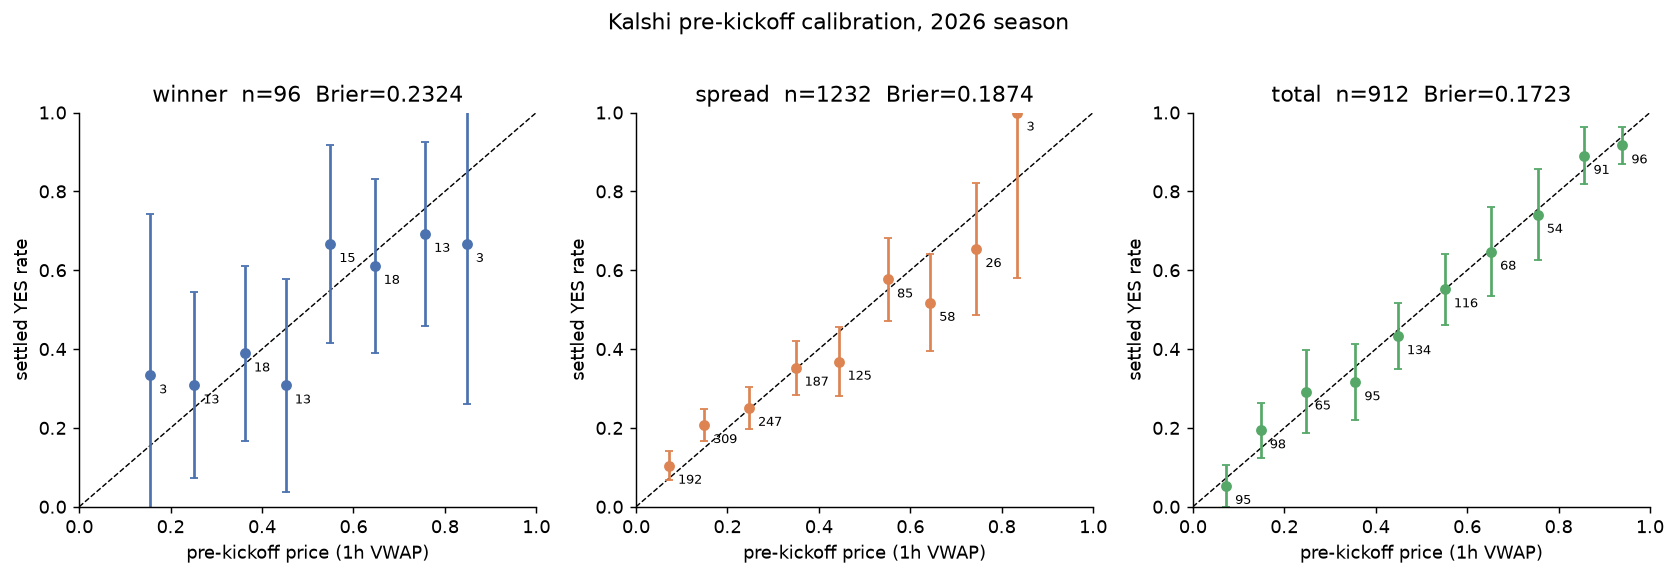
\includegraphics[width=0.95\textwidth]{kalshi_calibration.png}
\caption{Calibration of Kalshi pre-kickoff prices (1-hour volume-weighted average) against settlement, 2026 weeks 1--3, by contract type.}
\label{fig:kalshi_cal}
\end{figure}

\subsection{NFL results and the pre-game feature table}

Historical results, play-by-play, rosters, injury reports and closing lines come from the public nflverse project~\cite{nflverse}. From them we built a table of 7,548 games (1999--2026) with 805 columns, one row per game in home-team orientation (Table~\ref{tab:features}). All data is free.

\begin{table}[H]
\centering
\small
\begin{tabular}{p{2.2cm}rp{8.3cm}p{1.9cm}}
\toprule
\textbf{Group} & \textbf{Cols} & \textbf{Content} & \textbf{From} \\
\midrule
Team form & 604 & 20 offensive and 20 defensive efficiency statistics from play-by-play (EPA per play, success rate, pass and rush splits, explosive-play rate, yards per play, completion percentage over expected, turnovers, sacks, third-down rate, points per drive, neutral-script EPA), each over five windows (last 4, last 8, exponentially weighted, season to date, previous season), for home, away and the home-minus-away difference & 1999; CPOE 2006 \\
Ratings & 68 & Pre-game Elo (FiveThirtyEight recipe), exponentially weighted margin, opponent-adjusted margin & 1999 \\
Quarterback & 23 & Scheduled starter's weighted EPA per dropback, CPOE, sack and interception rates, career dropbacks, starter-change flag & 1999 \\
Injuries & 44 & Players Out/Doubtful and Questionable by position group; snap share of players now out & 2009; snaps 2013 \\
Situational & 31 & Rest, bye, short week, primetime, dome, surface, temperature, wind, divisional, playoff & 1999 \\
Market & 10 & Closing spread, total, moneylines; stored for benchmarking, never used as features & 1999 \\
Targets & 5 & Home score, away score, margin, total, home win & 1999 \\
\bottomrule
\end{tabular}
\caption{The pre-game feature table.}
\label{tab:features}
\end{table}

Every feature is computed from information dated before kickoff: rolling statistics are shifted by one game, Elo is the pre-update value, and injury counts come from the report filed before the game. Following Glickman and Stern~\cite{glickmanstern2017}, each team statistic enters as the home value, the away value and their difference. We test for leakage by perturbation: one game's play-level statistics are multiplied by ten and thirty points added to its score, the table is rebuilt, and the game's own 233 team features and Elo must be unchanged while the two teams' later games change. Six random games pass. The test earned its keep: the nflverse schedule carries two post-game fields, \texttt{result} and \texttt{total}, that equal the targets. A forest trained with them reported a margin error of 2.4 points with 85\% of its importance on those two columns; they were removed and the table re-scanned for any column correlated above 0.6 with a target.

\subsection{Testing}

All programs are implemented in Python in a shared repository and run locally or on Google Colab. Models are evaluated walk-forward by season, training on all seasons before $t$ and testing on season $t$, because games within a season are related through the teams.
